%%%%%%%%%%%%%%%%%%%%%%%%%%%%%%%%%%%%%%%%%
% Short Sectioned Assignment
% LaTeX Template
% Version 1.0 (5/5/12)
%
% This template has been downloaded from:
% http://www.LaTeXTemplates.com
%
% Original author:
% Frits Wenneker (http://www.howtotex.com)
%
% License:
% CC BY-NC-SA 3.0 (http://creativecommons.org/licenses/by-nc-sa/3.0/)
%
%%%%%%%%%%%%%%%%%%%%%%%%%%%%%%%%%%%%%%%%%

%----------------------------------------------------------------------------------------
%	PACKAGES AND OTHER DOCUMENT CONFIGURATIONS
%----------------------------------------------------------------------------------------

\documentclass[paper=a4, fontsize=11pt]{scrartcl} % A4 paper and 11pt font size
\usepackage{subcaption}
\usepackage{float}
\usepackage{listings}
\usepackage{amsmath}
\usepackage{color}

\definecolor{dkgreen}{rgb}{0,0.6,0}
\definecolor{gray}{rgb}{0.5,0.5,0.5}
\definecolor{mauve}{rgb}{0.58,0,0.82}

\lstset{frame=tb,
  language=MATLAB,
  aboveskip=3mm,
  belowskip=10mm,
  showstringspaces=false,
  columns=flexible,
  basicstyle={\small\ttfamily},
  numbers=none,
  numberstyle=\tiny\color{gray},
  keywordstyle=\color{blue},
  commentstyle=\color{dkgreen},
  stringstyle=\color{mauve},
  breaklines=true,
  breakatwhitespace=true,
  tabsize=3
}

\usepackage{CJKutf8} % chinese support
\usepackage{graphicx}

\usepackage[T1]{fontenc} % Use 8-bit encoding that has 256 glyphs
\usepackage{fourier} % Use the Adobe Utopia font for the document - comment this line to return to the LaTeX default
\usepackage[english]{babel} % English language/hyphenation
\usepackage{amsmath,amsfonts,amsthm} % Math packages

\usepackage{lipsum} % Used for inserting dummy 'Lorem ipsum' text into the template

\usepackage{sectsty} % Allows customizing section commands
\allsectionsfont{\centering \normalfont\scshape} % Make all sections centered, the default font and small caps

\usepackage{fancyhdr} % Custom headers and footers
\pagestyle{fancyplain} % Makes all pages in the document conform to the custom headers and footers
\fancyhead{} % No page header - if you want one, create it in the same way as the footers below
\fancyfoot[L]{} % Empty left footer
\fancyfoot[C]{} % Empty center footer
\fancyfoot[R]{\thepage} % Page numbering for right footer
\renewcommand{\headrulewidth}{0pt} % Remove header underlines
\renewcommand{\footrulewidth}{0pt} % Remove footer underlines
\setlength{\headheight}{13.6pt} % Customize the height of the header

\numberwithin{equation}{section} % Number equations within sections (i.e. 1.1, 1.2, 2.1, 2.2 instead of 1, 2, 3, 4)
\numberwithin{figure}{section} % Number figures within sections (i.e. 1.1, 1.2, 2.1, 2.2 instead of 1, 2, 3, 4)
\numberwithin{table}{section} % Number tables within sections (i.e. 1.1, 1.2, 2.1, 2.2 instead of 1, 2, 3, 4)

\setlength\parindent{0pt} % Removes all indentation from paragraphs - comment this line for an assignment with lots of text

%----------------------------------------------------------------------------------------
%	TITLE SECTION
%----------------------------------------------------------------------------------------

\newcommand{\horrule}[1]{\rule{\linewidth}{#1}} % Create horizontal rule command with 1 argument of height

\title{
\normalfont \normalsize 
\textsc{计算物理学15春季} \\ [25pt] % Your university, school and/or department name(s)
\horrule{0.5pt} \\[0.4cm] % Thin top horizontal rule
\huge 第四次作业解题报告 \\ % The assignment title
\horrule{2pt} \\[0.5cm] % Thick bottom horizontal rule
}

\author{霍浩岩} % Your name

\date{\normalsize\today} % Today's date or a custom date

\begin{document}
\begin{CJK*}{UTF8}{gbsn}

\maketitle % Print the title

%----------------------------------------------------------------------------------------
%	PROBLEM 1
%----------------------------------------------------------------------------------------

\section{Wave Function}

\subsection{推导过程}

需要求解的波函数偏微分方程的形式为:

\begin{equation}
\frac{\partial u}{\partial t}+c\frac{\partial u}{\partial x}=0 
\end{equation}

其中$c$是波速。将波动方程在求解区间上分割为$u_0,u_1,\dots,u_N$的等距点,并采用周期性边界条件:
\begin{equation}
u_0 = u_N
\end{equation}
这样偏微分方程就可以写成线性方程组的形式
\begin{equation}
u_j^{n+1}=u_j^n-\frac{c\Delta t}{\Delta x}(u_j^n-u_{j-1}^n), j=0,1,\dots,N \\\\
\end{equation}
取$r=\frac{c\Delta t}{\Delta x}$,将这一组方程写成矩阵乘法的形式:
\begin{equation}
\begin{bmatrix}
u_0^{n+1} \\\\ u_1^{n+1} \\\\ \vdots \\\\ u_N^{n+1} 
\end{bmatrix} = \begin{bmatrix}
1-r & 0 & \dots & r \\\\
r & 1-r & \dots & 0 \\\\
\vdots & \ddots & \ddots & \vdots \\\\
0 & \dots & r & 1-r
\end{bmatrix} \begin{bmatrix}
u_0^n \\\\ u_1^n \\\\ \vdots \\\\ u_N^n 
\end{bmatrix}
\end{equation}

\subsection{程序求解}

将上面的矩阵用MATLAB语言编写成求解程序:
\lstset{language=MATLAB}
\begin{lstlisting}
% upwind.m, a function implements upwind scheme 
function upwind(init, r)
                                % make a column vector
  u = init(:);
  N = size(u, 1);

                                % A matrix (sparse)
  A = spdiags(repmat([1-r r], N), [0 -1], N, N);
  A(1,N) = r;

  for j=1:10000
    plot(u);

                                % adjust axis
    a = axis;
    axis([0 N a(3) a(4)]);
    xlabel('x');
    ylabel('u');
    text(0.8*N, 0.8*(a(4)-a(3)+a(3)), sprintf('step: %d', j));

                                % update u vector
    u = A*u;

    pause(0.01);
  end
end
\end{lstlisting}


选取初始条件为正弦波函数,即调用上述函数的方法为:
\lstset{language=MATLAB}
\begin{lstlisting}
upwind(sin([0:0.1:2*pi]), 0.4);
\end{lstlisting}

这是$r=0.4$的情形。为了观察波函数的演化过程,将不同时间($j=1,21,41,\dots,101$)的波函数画在同一张图上,如图Figure 1.1。让$r=1$和$r=1.5$,画出不同情况下的波函数演化图,如图Figure 1.2、Figure 1.3。\\\\
\begin{figure}[H]
\centering
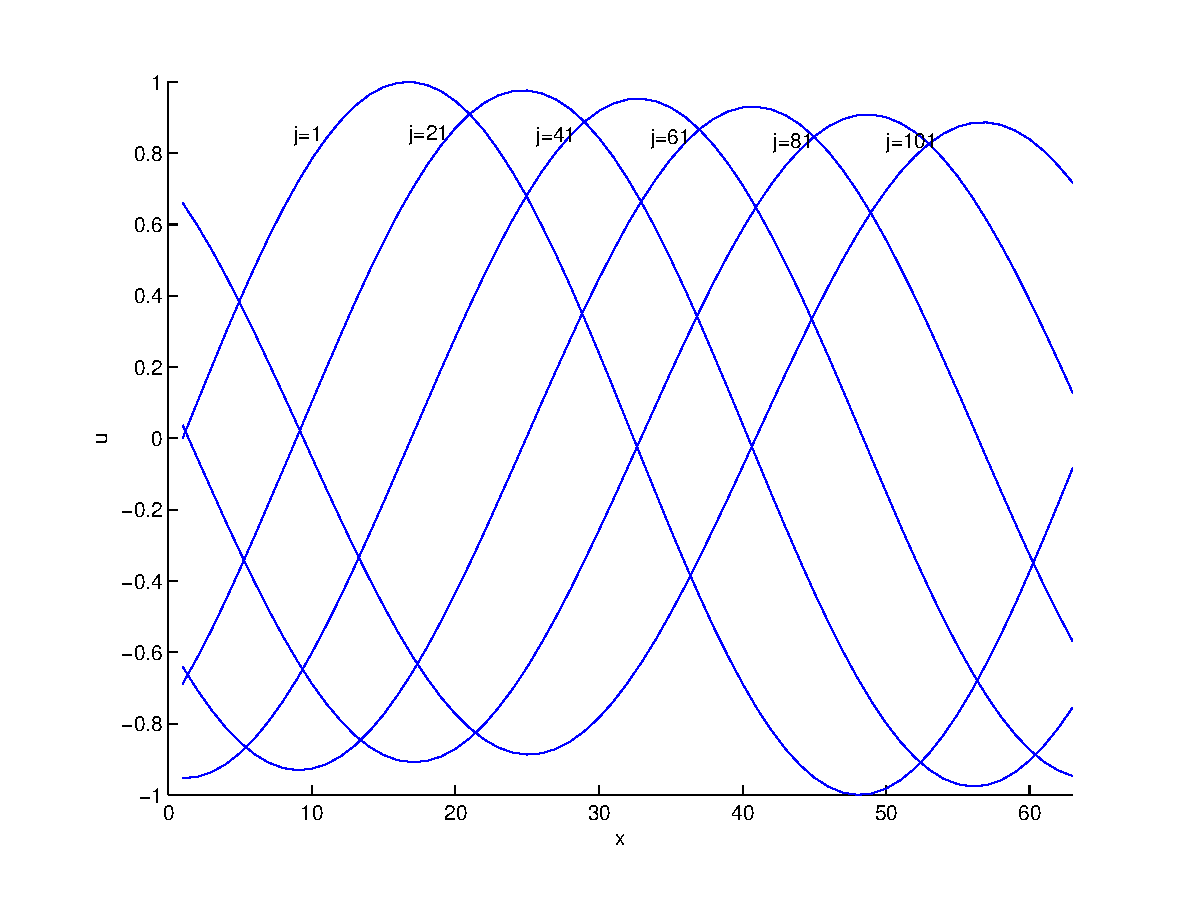
\includegraphics[width=90mm]{figure1-1.eps}
\caption{波函数的演化,Œ–$r=0.4$}
\end{figure}

\begin{figure}[H]
\centering
\begin{subfigure}{70mm}
  \centering
  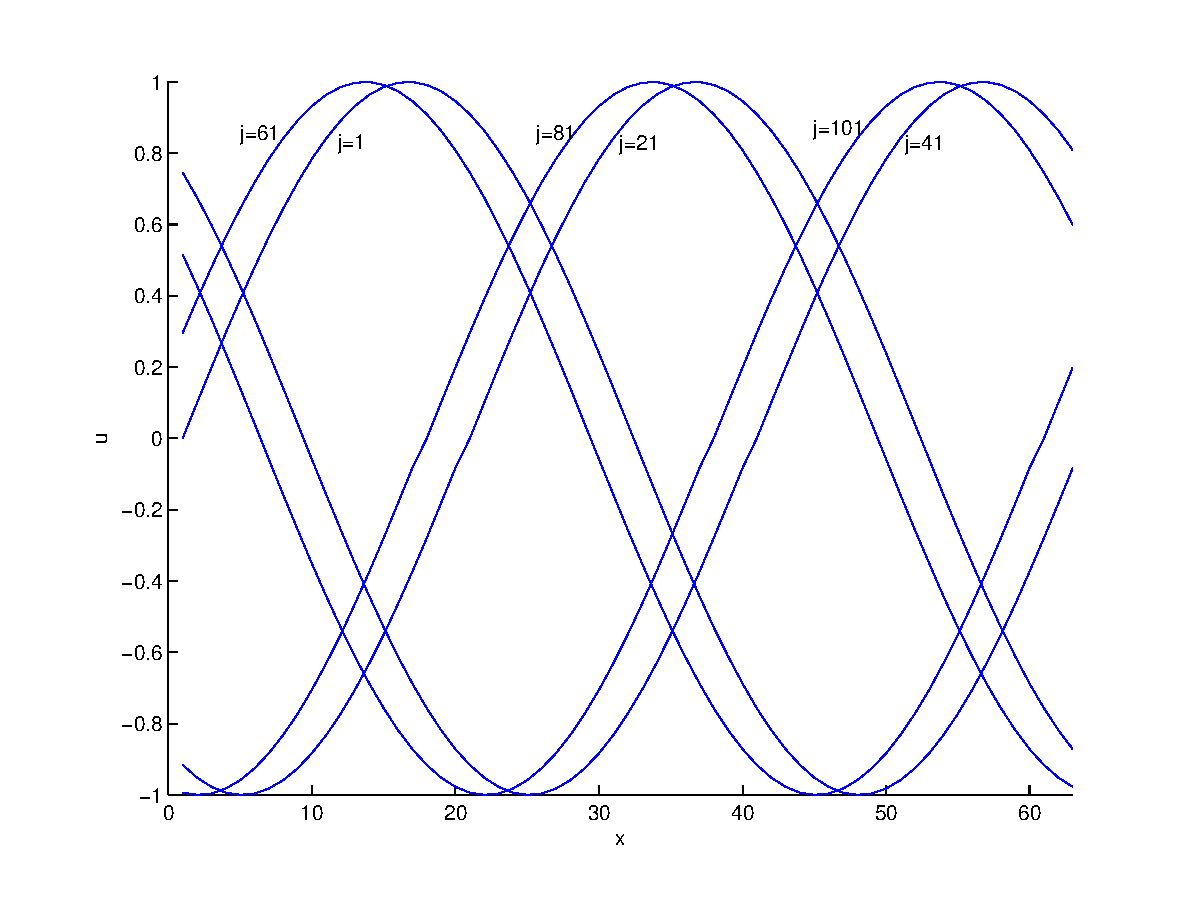
\includegraphics[width=65mm]{figure1-2.eps}
  \caption{$r=1.0$}
  \label{fig:sub1}
\end{subfigure}
\begin{subfigure}{70mm}
  \centering
  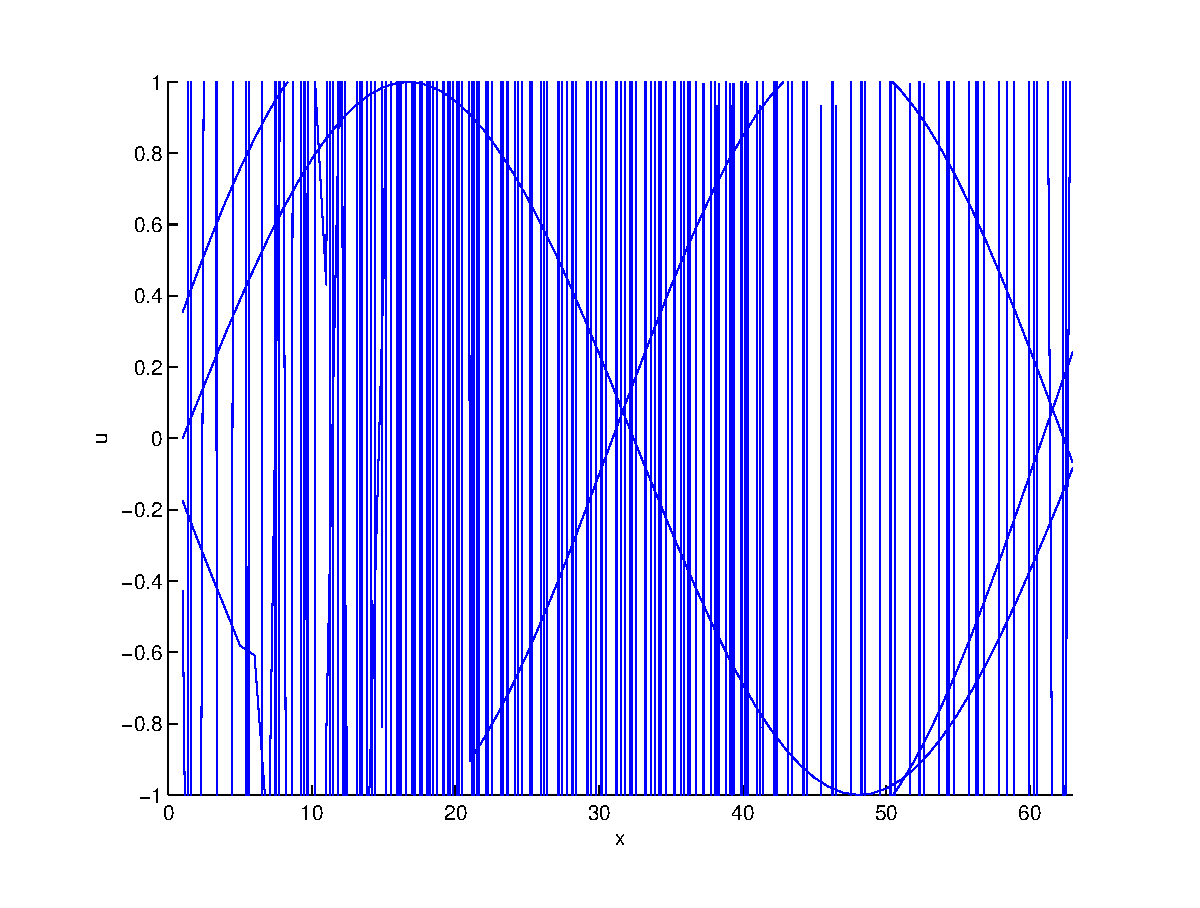
\includegraphics[width=65mm]{figure1-3.eps}
  \caption{$r=1.5$}
  \label{fig:sub2}
\end{subfigure}
\caption{不同$r$的求解}
\label{fig:test}
\end{figure}


可以看到,Figure 1.1中,波函数的峰峰值不断下降,事实上我们的波动方程中并没有衰减项,矩阵解法的精度是有限的(采用有限步长近似实际上为方程加入了非线性项,导致解衰减)。其次可以发现$r$的选取对解的性质有很大的影响:如果$r$选择过大解就会发散;然而$r$的值和波速$c$有关,因此在不同的波速下需要选择不同的时间步长才能得到合适的解。

\pagebreak
\section{Boundary value problem}
\subsection{提出方程}
$y$方向具有周期性边界条件,$x$方向有第一类边界条件的二维泊松方程写作:

\begin{equation}
\frac{\partial^2 u}{\partial x^2}+\frac{\partial^2 u}{\partial y^2}=\rho(x,y) ,x\in[0, 1], y\in[0, 1] 
\end{equation}
\begin{equation}
u(x, 0) = u(x, a)
\end{equation}
\begin{equation}
u(0,y) = Y_0(y)
\end{equation}
\begin{equation}
u(1,y) = Y_1(y)
\end{equation}

将求解区域的$x,y$方向分别分割成$N_x,N_y$个点,在格点$(i,j)$处,泊松方程是:
\begin{equation}
\frac{2u(i,j)-u(i-1,j)-u(i+1,j)}{\Delta x^2}+\frac{2u(i,j)-u(i,j-1)-u(i,j+1)}{\Delta y^2}=\rho(i,j)
\end{equation}
在$y$方向上进行傅立叶变换,并考虑到周期性边界条件$u(i,0)=u(i,N_y)$:
\begin{equation}
\sum_{j=1}^{N_y}e^{i\frac{2\pi}{N_y}k(j-1)}\rho(i,j) = g(i,k)
\end{equation}
\begin{equation}
\sum_{j=1}^{N_y}e^{i\frac{2\pi}{N_y}k(j-1)}u(i,j) = f(i,k)
\end{equation}
\begin{equation}
\sum_{j=1}^{N_y}e^{i\frac{2\pi}{N_y}k(j-1)}u(i,j-1) = e^{i\frac{2\pi}{N_y}k} f(i,k)
\end{equation}
\begin{equation}
\sum_{j=1}^{N_y}e^{i\frac{2\pi}{N_y}k(j-1)}u(i,j+1) = e^{-i\frac{2\pi}{N_y}k} f(i,k)
\end{equation}
$x$的左右边界同样通过傅立叶变换变换成序列$f_0(k)$和$f_1(k)$。根据上面三个式子,再结合之前的一维微分方程的矩阵解法,可以重新将二维泊松方程写成:
\begin{equation}
(\mathbf{A}-\frac{1}{\Delta y^2}4sin^2(\frac{\pi}{N_y}k) \mathbf{I}) \begin{bmatrix}
f(2, k) \\\\ f(3, k) \\\\ \vdots \\\\ f(N_x-1, k) \end{bmatrix} = \frac{1}{\Delta x^2} \begin{bmatrix} f_0(k) \\\\ 0 \\\\ \vdots \\\\ f_1(k) \end{bmatrix} + \begin{bmatrix} g(2, k) \\\\ g(3,k) \\\\ \vdots \\\\ g(N_x-1, k) \end{bmatrix}
\end{equation} 
其中,
\begin{equation}
\mathbf{A} = \frac{1}{\Delta x^2}\begin{bmatrix}
2 & -1 \\\\
-1 & 2 & -1 \\\\
 & \ddots & \ddots & \ddots \\\\
 & & -1 & 2 & -1 \\\\
 & & & -1 & 2
 \end{bmatrix}
\end{equation}
根据上面的一维方程求出$u(i,k)$之后,再根据逆傅立叶变换求出泊松方程的解:
\begin{equation}
\frac{1}{N_y}\sum_{k=1}^{N_y}e^{-i\frac{2\pi}{N_y}j(k-1)}f(i,k) = u(i,j)
\end{equation}


\subsection{问题求解}
使用MATLAB编写求解上述二维泊松方程的程序,如下:
\lstset{language=MATLAB}
\begin{lstlisting}
%%%%%%%%%%%%%%%%%%%%%%%%%%%%%%%%%%%%%%%%
% function fourier_solve, a demonstration of 
% solving possion PDE using fourier seris
%
%%%%%%%%%%%%%%%%%%%%%%%%%%%%%%%%%%%%%%%%
function fourier_solve()
                   % x: left_border:0, right_border:1, source:1/(NX+1)->NX/(NX+1)
                   % y: source: 0->(NY-1)/NY
                   % dx=1/(NX+1), dy=1/NY
  NY = 100;
  NX = 10;

  dx = 1/(NX+1);
  dy = 1/NY;

                                % fill left/right border and source
  left = transpose(border_left_function([0:NY-1]*dy));
  right = transpose(border_right_function([0:NY-1]*dy));
  [mesh_x, mesh_y] = meshgrid([1:NX]*dx,[0:NY-1]*dy);
  source = source_function(mesh_x, mesh_y);

                                % transform them into fourier seris
  left_f = fourier(left);
  right_f = fourier(right);
  source_f = fourier(source);

                                % solve 1d problems under parameter k
  u = zeros(NY, NX);
  for j=1:NY
    u(j,:) = solve_1d(source_f(j,:), left_f(j), right_f(j), NX, NY, dx, dy, j-1);
  end

                                % transform back
  u = reverse_fourier(u);

  figure;
  imagesc(real(u));
  xlabel('x');
  ylabel('y');
  title('solution');
  colorbar;

  figure;
  imagesc(solution_function(mesh_x, mesh_y));
  xlabel('x');
  ylabel('y');
  title('original solution')
  colorbar;
end

%%%%%%%%%%%%%%%%%%%%%%%%%%%%%%%%%%%%%%%%
% test case
%%%%%%%%%%%%%%%%%%%%%%%%%%%%%%%%%%%%%%%%
function u=solution_function(x,y)
                                % test case 1
  % u = x.^2;

                                % test case 2
  % u = sin(2*pi*y);

                                % test case 3
  u = sin(2*pi*y).*(1-x)+ x.*cos(2*pi*y);
end
function u=border_left_function(y)
                                % test case 1
  % u = 0*y;

                                % test case 2
  % u = sin(2*pi*y);

                                % test case 3
  u = sin(2*pi*y);
end
function u=border_right_function(y)
                                % test case 1
  % u = 1 * ones(1, size(y(:), 1));

                                % test case 2
  % u = sin(2*pi*y);

                                % test case 3
  u = cos(2*pi*y);
end
function u=source_function(x,y)
                                % test case 1
  % u = ones(size(x,1),size(x,2));

                                % test case 2
  % u = -4*pi^2*sin(2*pi*y);

                                % test case 3
  u = -4*pi^2*(sin(2*pi*y).*(1-x)+ x.*cos(2*pi*y));
end
%%%%%%%%%%%%%%%%%%%%%%%%%%%%%%%%%%%%%%%%
% test case end
%%%%%%%%%%%%%%%%%%%%%%%%%%%%%%%%%%%%%%%%

%%%%%%%%%%%%%%%%%%%%%%%%%%%%%%%%%%%%%%%%
% solve 1d problem d^2u/dx^2 - 4sin(pi*k/NY)^2 u = rho(x)
%
% source: NX-by-1 matrix
% left: numeric, left border condition
% right: numeric, right border condition
% NX, NY: integer,
% dx: numeric
% k: numeric
%%%%%%%%%%%%%%%%%%%%%%%%%%%%%%%%%%%%%%%%
function u = solve_1d(source, left, right, NX, NY, dx, dy, k)
  A = spdiags(repmat([-1 2 -1], NX, 1), [1 0 -1], NX, NX) / dx^2;
  B = A - 4*(sin(pi/NY*k))^2 / dy^2 * eye(NX);

  b = zeros(NX, 1);
  b(1) = left / dx^2;
  b(NX) = right / dx^2;
  b = b + source(:);

  u = B \ b;
end

%%%%%%%%%%%%%%%%%%%%%%%%%%%%%%%%%%%%%%%%
% transform a list of vectors into its fourier seris
%
% input: N-by-M matrix of M vectors to transform
%%%%%%%%%%%%%%%%%%%%%%%%%%%%%%%%%%%%%%%%
function output=fourier(input)
  N = size(input, 1);

  A = ones(N);

  K = 2*pi/N;
  for j=1:N
    for k=1:N
      A(j,k) = exp((j-1)*(k-1)*i*K);
    end
  end

  output = zeros(size(input,1),size(input,2));
  for j=1:size(input,2)
    output(:,j) = A*input(:,j);
  end
end

%%%%%%%%%%%%%%%%%%%%%%%%%%%%%%%%%%%%%%%%
% transform a list of fourier seris back
%
% input: N-by-M matrix of M vectors to transform
%%%%%%%%%%%%%%%%%%%%%%%%%%%%%%%%%%%%%%%%
function output=reverse_fourier(input)
  N = size(input, 1);

  A = ones(N);

  K = 2*pi/N;
  for j=1:N
    for k=1:N
      A(j,k) = exp(-(j-1)*(k-1)*i*K) / N;
    end
  end

  output = zeros(size(input,1),size(input,2));
  for j=1:size(input,2)
    output(:,j) = A*input(:,j);
  end
end

\end{lstlisting}
上面的程序中,共提出了三种测试用的解析解,使用解为$u(x,y)=sin(2\pi y)(1-x)+ xcos(2\pi y)$的测试用例求解结果如下(为了便于打印已将imagesc函数换成contour函数):

\begin{figure}[H]
\centering
\begin{subfigure}{70mm}
  \centering
  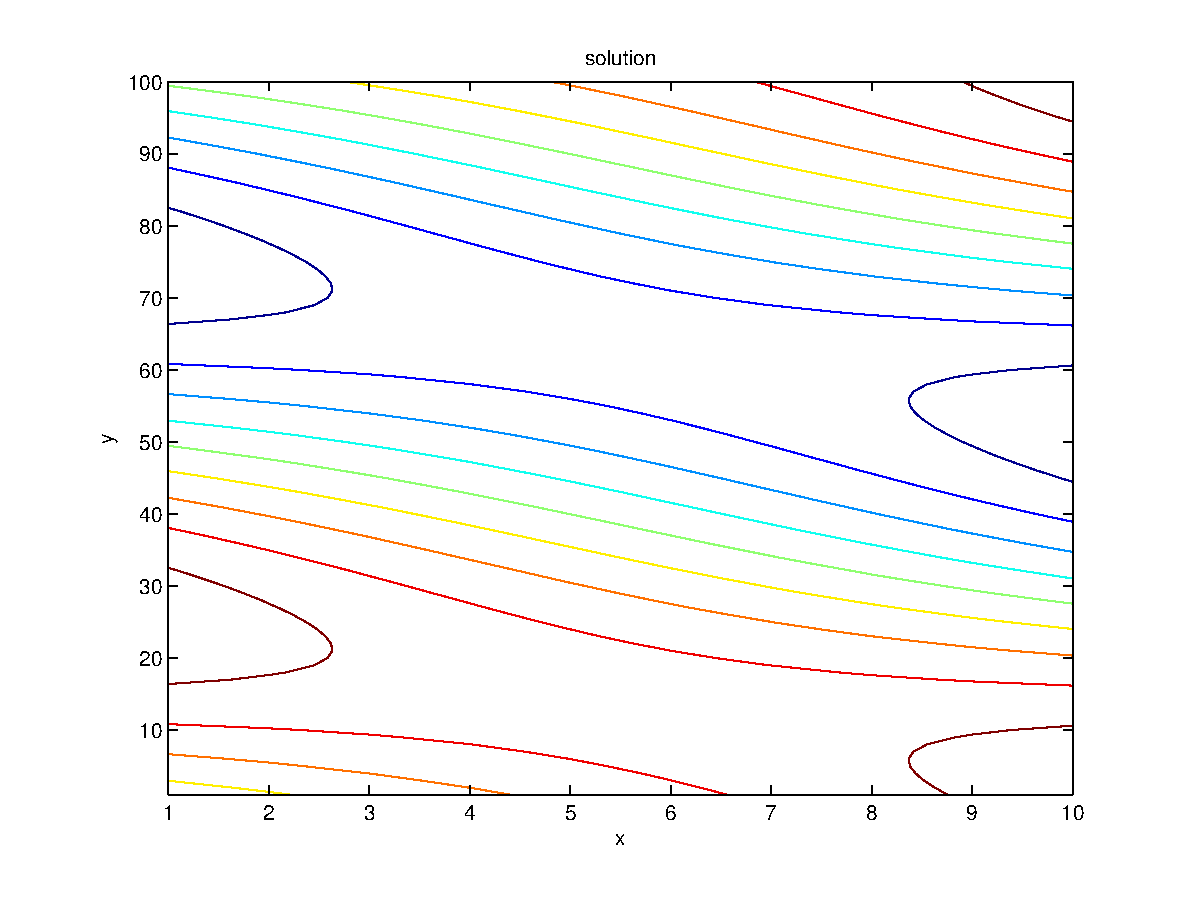
\includegraphics[width=65mm]{figure-2-1-1.eps}
  \caption{程序求出的解}
  \label{fig:sub1}
\end{subfigure}
\begin{subfigure}{70mm}
  \centering
  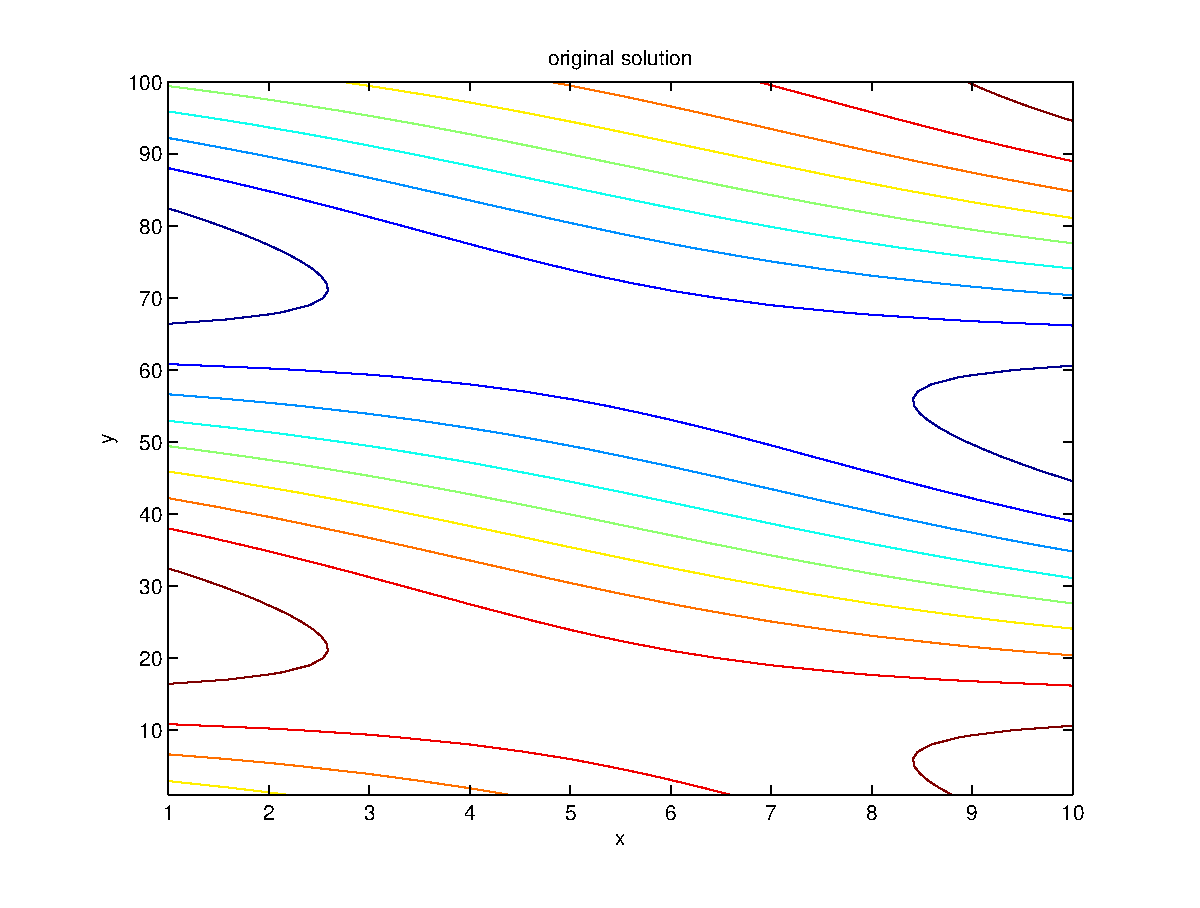
\includegraphics[width=65mm]{figure-2-1-2.eps}
  \caption{解析解}
  \label{fig:sub2}
\end{subfigure}
\caption{二维泊松方程求解}
\label{fig:test}
\end{figure}

\subsection{遇到的问题}
对复矩阵进行转置(transpose)的操作会求矩阵的转置后再取复共轭,这常常会导致不可预料的错误,因此应该使用下面的代码将行矩阵转换成列矩阵
\lstset{language=MATLAB}
\begin{lstlisting}
m = m(:)
\end{lstlisting}
另外,为了避免不必要的计算,可以将傅立叶变换矩阵求出后存入静态变量。但是由于目前不是十分了解MATLAB编程语言,暂时没有找到合适的方法。

最后,选择测试用例的时候需要特别注意,测试用例的$y$方向上由于需要满足周期性边界条件,因此必须保证在端点处的函数值和导数连续,否则就无法求解。
%----------------------------------------------------------------------------------------
\end{CJK*}
\end{document}
